\documentclass[12pt,a4paper]{article}

\usepackage[top=2.5cm,bottom=2cm,left=2cm,right=2cm]{geometry} 
\usepackage[brazil]{babel}
\usepackage{blindtext}
\usepackage{ragged2e}
\usepackage[utf8]{inputenc}
\usepackage{indentfirst}
\usepackage{mathtools}
\setlength\parindent{24pt}

%capa
\usepackage{multicol}
\usepackage{multirow}
\usepackage{graphicx}
\usepackage{float}
\usepackage{setspace} % espaçamento
\usepackage{tabularx}
\usepackage{booktabs}
\usepackage{array}


\newcommand{\university}{Universidade de São Paulo - ICMC}
\newcommand{\discipline}{SCC0530 - Inteligência Artificial}
\newcommand{\data}{$1^o$ semestre / 2018}
\newcommand{\teacher}{Prof. Solange Oliveira Rezende}
\newcommand{\PAE}{PAEs: Felipe Provezano Coutinho }
\newcommand{\specification}{Busca de caminho em um Sliding Puzzle}

\newcommand{\members}{
    \begin{table}[!ht]
        \centering
        \begin{tabular}{ll}
            \large\textsc{Gabriel Simmel Nascimento} & \large\textsc{Nº USP: 9050232} \\
            \large\textsc{Giovanna Oliveira Guimarães} & \large\textsc{Nº USP: 9293693} \\
            \large\textsc{José Augusto Noronha de Menezes Neto} & \large\textsc{Nº USP: 9293049} \\
            \large\textsc{Julia Diniz Ferreira} & \large\textsc{Nº USP: 9364865} \\
            \large\textsc{Lucas Alexandre Soares} & \large\textsc{Nº USP: 9293265} \\
            \large\textsc{Otávio Luis Aguiar} & \large\textsc{Nº USP: 9293518} \\
            \large\textsc{Rafael Augusto Monteiro} & \large\textsc{Nº USP: 9293095} \\
        \end{tabular}
    \end{table}{}
}

\newcommand{\capaicmc}{
    \begin{center}
        \begin{center}
            \begin{table}[!ht]
                \centering 
                \begin{tabular}{cl}
                    \multirow{4}{*}{
\includegraphics[height=1.8cm,keepaspectratio=true]{logo-header.png}}
                    & \university\\
                    %& \course\\ 
                    & \discipline\\
                    & \teacher\\
                    %& \PAE\\
                \end{tabular}
            \end{table}
        \end{center}
        
        \vfill
        
        {\huge \specification}
        
        \vfill
        
        \doublespacing
        \large\textsc{\members}
        
        \vfill
        
        \large São Carlos - SP \\
        \large \today \\

        \end{center}
        
        \newpage
}

\begin{document}

% Capa
\capaicmc

\tableofcontents
\newpage

% Seta espaçamento entre linhas
\singlespacing

% Introdução: Explicar o problema, dar uma descrita rápida em como vamos abordar o problema. Talvez fosse legal explicar sobre como esse documento está estruturado.
\section{Introdução}
O problema tratado neste projeto é a busca de um caminho para resolver um tabuleiro do jogo \textit{Sliding Puzzle}. O jogo consiste em um tabuleiro $N$ por $N$, onde $N$ é um inteiro maior que 1, de peças deslizantes, que precisam ser arranjadas de forma a encontrar uma configuração específica. Para atingir o estado final, deve-se deslizar peças para o espaço vazio. A imagem 1 exemplifica um tabuleiro em seu estado inicial, enquanto a imagem 2 exemplifica o tabuleiro no estado final. \par

%alguém arruma essas imagens, coloca legenda e os carai por favor
\begin{center}
    %legenda: Imagem 1: Um possível estado inicial do tabuleiro
    \includegraphics[height=3cm]{wrong.png}
    %legenda: Imagem 2: Estado final buscado.
    \includegraphics[height=3cm]{right.PNG}
\end{center} \par

Uma solução para o problema é um caminho, isto é, um conjunto de passos que podem ser dados para atingir o estado alvo. Modelando o problema como uma busca em árvore, é possível utilizar algoritmos de busca para encontrar um caminho ótimo. Nas sessões seguintes, descreveremos mais profundamente a modelagem do problema e os algoritmos utilizados. \par

\newpage
% Métodos: Explicar como fizemos pra resolver o problema
\section{Métodos}
% Modelagem: Explicar como modelamos o jogo em um problema de busca. Falar como o espaço de busca é grande
\subsection{Modelagem}
    \par Com o objetivo de encontrar um método genérico para solucionar os \textit{puzzles}, implementamos um grafo no qual cada um de seus nós consiste nos estados possíveis de um tabuleiro qualquer. As Figuras 1 e 2, por exemplo, representam dois nós de um destes grafos, sendo a Figura 1 o nó inicial e a 2 o nó alvo (final).
    \par Os nós adjacentes representam os estados que podem ser alcançados a partir do nó atual ao "movimentar" o espaço vazio do tabuleiro para qualquer posição válida. Ou seja, se a lacuna encontra-se em uma posição na qual há quatro possibilidades válidas de movimento, o vértice correspondente a configuração atual terá quatro nós vizinhos.
    \par Embora trate-se de um problema aparentemente simples, o desenvolvimento de uma algorítimo capaz de apresentar uma solução para um caso genérico não é uma tarefa trivial, devido à complexidade do espaço de busca. Por exemplo, o caso de um jogo de dimensões 4x4:
    \begin{itemize}
    \item Cada uma das peças pode ocupar qualquer posição do tabuleiro;
    \item Para cada posição que uma peça ocupa, as demais também podem alternar-se entre os demais espaços disponíveis.
    \end{itemize}
    \par Dado isto, vemos que a complexidade do espaço de busca é fatorial e, por isso, mesmo para jogos cujas medidas são pequenas, o espaço obtido terá dimensões extremamente grandes. Tal como no caso apresentado, que possui um total de $2.092279 e^{1   3}$ estados válidos.  \par
    Ainda, com o intuito de reduzir o espaço de busca, limitamos para casos onde o caminho mínimo possui no máximo 45 passos. 

% Algoritmos de busca: Explicar os algoritmos utilizados
\subsection{Algoritmos de Busca}
Nesta sessão, serão descritos os algoritmos de busca implementados para a resolução do problema de busca apresentado acima. 

% A*: Explicar como o A* funciona
\subsubsection{A*}
\par O A* é um algorítimo de busca informada, que percorre o espaço de busca a procura da solução que apresentar menor custo para o problema em questão. O algorítimo considera, dentre as possibilidades, primeiramente as que, ao que tudo indica, são a melhor opção no momento. A cada iteração, o A* determina quais de suas pré soluções deverão ser expandidas, o que é feito com base em uma estimativa do custo necessário para que o objetivo seja atingido. Em suma, o A* escolhe as soluções que minimizem a função:
\[f(n)=g(n)+h(n)\]
\par Onde $n$ é o último nó adicionado à solução, $g(n)$ é o custo da solução desde o nó inicial até $n$ e $h(n)$ uma heurística admissível que estima o custo da solução mais barata de $n$ até o objetivo final.
\par Para o cenário de um \textit{15 Sliding Puzzle Game}, a distância de Manhattan é uma heurística $h(n)$ admissível, isto é:
\[h(n) \leq h*(n)\]
\par Para todos os nós $n$, onde $h^{*}$ é o custo real da melhor solução de $n$ para o objetivo final.
\par Ao utilizarmos uma heurística admissível, a solução encontrada pelo A* será sempre ótima. Para $g(n)$, nosso algorítimo considera o custo de se realizar um movimento válido no tabuleiro, ou seja, partir do nó atual (estado imediato) para algum de seus vizinhos (estados válidos alcançáveis).
\par Com o objetivo de reduzir o número de operações realizadas pelo algorítimo, a cada passo realizado, é feita uma checagem para garantir que o A* nunca retorne ao estado do qual acabara de sair.
% IDA*: Explicar como o IDA* funciona
\subsubsection{IDA*}

\par O IDA*, \textit{Iterative-deepening-A*}, performa, a cada iteração, uma busca de primeira profundidade. Ou seja, quando o custo total de uma solução, $f(n)$, excede um dado limite de profundidade, o IDA* interrompe, momentânea ou permanentemente, o processamento de tal solução. O cálculo deste limite tem início com a estimativa do custo no estado inicial da busca e aumenta a cada iteração do algorítimo. A cada passo do \textit{loop}, o limite utilizado para o próximo é o custo mínimo dentre todos os valores que excedem limiar atual.
\par Tal como o A* descrito anteriormente, o IDA* também garante que a solução encontrada é a solução ótima, desde que seja escolhida uma heurística admissível para o contexto do problema.
%Sua vantagem em relação ao A* está atrelada à utilização de memória, uma vez que este mantém uma fila de nós inexplorados que pode crescer rapidamente e ocupar uma grande parte da memória disponível. Já o IDA* possui uma demanda linear de memória, visto que armazena nenhum outro nó que não seja o atual.

% Programa: Falar um pouco sobre quais as entradas que o programa recebe, quais as saídas geradas, como rodar e quais os requisitos
\subsection{Programa}
\subsubsection{Descrição}
    \par Dois programas foram feitos em linguagem C++, um para cada algoritmo, cada um em um arquivo {\it .zip}. Ambos os programas recebem a mesma entrada: 16 valores inteiros separados por espaços e/ou quebra de linhas, e suas saídas são o tempo de execução, o número de iterações e a sequência de passos que resolve o tabuleiro.
    Para compilar e rodar os programas, um Makefile está incluso em cada arquivo {\it .zip}, basta executar \verb|make| e \verb|make run|.

\newpage
% Resultados: Falar dos resultados obtidos
\section{Resultados}

% Execuções: Mostrar uma tabela com os resultados das execuções.
\subsection{Execuções}
    \par A tabela 1 apresenta o tempo médio de dez execuções dos algoritmos para quatro tabuleiros com as seguintes configurações:

% colocar imagem do tabuleiro usado nos testes
\begin{center}
    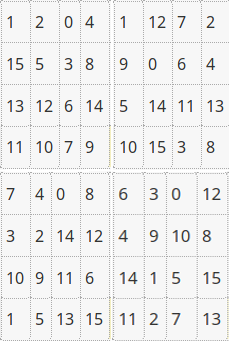
\includegraphics{test-puzzles.png}
\end{center}

% Por favor, alguém coloca uma legenda nessa tabela
\begin{center}
    \begin{tabular}{c|r|r|}
        \cline{2-3}
        & \multicolumn{2}{c|}{Tempo de Execução} \\
        \cline{2-3}
        & IDA* & A* \\
        \cline{2-3}
        \hline
        \multicolumn{1}{|c|}{Média caso 1} & $ 0.001365 $ & $ 0.052758 $ \\
        \hline
        \multicolumn{1}{|c|}{Desvio caso 1} & $ 0.000234 $ & $ 0.003331 $ \\
        \hline
        \multicolumn{1}{|c|}{Média caso 2} & $ 0.597372 $ & $ 3.655886 $ \\
        \hline
        \multicolumn{1}{|c|}{Desvio caso 2} & $ 0.002716 $ & $ 0.045991 $ \\
        \hline
        \multicolumn{1}{|c|}{Média caso 3} & $ 0.001580 $ & $ 0.238017 $ \\
        \hline
        \multicolumn{1}{|c|}{Desvio caso 3} & $ 0.000033 $ & $ 0.008325 $ \\
        \hline
        \multicolumn{1}{|c|}{Média caso 4} & $ 2.736517 $ & Memória da máquina excedida \\
        \hline
        \multicolumn{1}{|c|}{Desvio caso 4} & $ 0.041999 $ & Memória da máquina excedida \\
        \hline
    \end{tabular}
\end{center} \par

% Discussão: Discutir sobre os resultados. Falar por que o IDA* é melhor que o A*, etc.
\subsection{Discussão}

    \par Apesar de possuírem uma complexidade temporal equivalente, o IDA* possui uma menor complexidade espacial. Por manter uma fila com os nós ainda não explorados, o A* pode rapidamente consumir boa parte da memória disponível para execução do programa, pois, em seu pior caso, haverá um número exponencial de nós. Já o IDA* possui uma demanda linear de memória, visto que não armazena nenhum outro nó que não seja o atual. Como podemos ver na tabela, o A* não foi capaz de resolver um dos testes por dar erro de memória, mostrando que, de fato, o A* consome muito mais memória. Este comsumo maior de memória implica em mais custos de tempo também devido à necessidade de manter e manejar os nós já visitados, tornando-o mais lento que o IDA* no caso geral.
    \par A princípio, os algorítimos foram implementados em \textit{python} em função da simplicidade da linguagem, contudo, o custo de utilizar uma linguagem de tão alto nível, causou um impacto muito grande em consumo de memória e {\it overhead} em tempo. Isto tornou a execução dos casos testes inviável e, por fim, optamos por uma implementação em C++.

\newpage

% Conclusão: Resumir o que foi discutido na sessão de discussão e dar uma conclusão, dizendo que o IDA* é melhor que o A* pra esse problema.
\section{Conclusão}
    \par Por fim, pode-se concluir que, para nosso o problema, o IDA* mostra-se como uma alternativa superior ao A*, dado que seu consumo de memória é muito menor (linear contra exponencial) que causa um impacto grande na performance de casos mais complexos.
    \par Além disso, notamos que \textit{python} não é uma linguagem apropriada para este cenário específico, uma vez que, por ser de muito alto nível, ela não oferece recursos necessários para que os algorítimos desenvolvidos sejam executados em um intervalo de tempo aceitável.
\newpage

\section{Extra}
No início, começamos a implementar os algoritmos em Python. Porém, a execução mostrou-se muito custosa, devido ao \textit{overhead} de operações em listas e criação de objetos. Em seguida, reimplementamos os algoritmos em C++, que se mostrou muito mais rápido. Os scripts gerados foram incluídos na submissão, na pasta "Extra". Para sua execução, é necessário a biblioteca Numpy e a versão 3 do Python.
\newpage
\end{document}